\subsection{Réseau}
\label{subsection:res}

Dans les sections \ref{subsubsection:fonctionnement_reseau} et \ref{subsection:network_implementaion}, nous avons présenté l'organisation et l'implémentation du réseau de communications de Simterpose. Nous voulons maintenant évaluer les performances de notre implémentation à travers divers tests.

\subsubsection{Protocole expérimental}
L'objectif principal étant de montrer qu'il est possible de faire de la virtualisation légère, nous souhaitons d'abord mesurer l'\textit{overhead} dû à l'utilisation de Simterpose. Dans un second temps, nous souhaitons mesurer les performances des deux types de médiations que nous avons implémentés. Cela nous permettrait de savoir quel type de médiation est le mieux adapté à l'application que l'on voulons exécuter.

Pour effectuer nos expériences, nous avons choisi deux applications réseau d'échanges de messages. La première application consiste à faire communiquer un client et un serveur en envoyant au serveur un million de messages de petite taille. On en envoie un million pour pallier le manque de précisions des \textit{timers}. La seconde va envoyer depuis un client un message de 1Mo à un serveur. Le protocole pour chaque expérience a été d'exécuter 20 fois chaque application en utilisant les mêmes appels systèmes pour communiquer les messages (\texttt{sendto}/\texttt{recvfrom} et \texttt{sendmsg}/\texttt{recvmsg}), puis une moyenne du temps d'exécution ainsi qu'une mesure des temps minimum et maximum ont été calculés.

\subsubsection{Résultats}
\paragraph{Overhead concernant le temps d'exécution}
Afin de mesurer l'\textit{overhead} produit par Simterpose, notre expérience consiste à exécuter les deux applications réseaux choisies sur une machine en utilisant uniquement le réseau local puis en utilisant Simterpose en suivant le protocole présenté plus haut. Ainsi, en comparant les temps d'exécution des applications sur les deux types d'architecture nous pourrons calculer l'\textit{overhead}. Les résultats de ces expériences sont présentés Figures \ref{Network_Big_Local} et \ref{Network_Little_Local}. L'histogramme représentant Simterpose correspond à la moyenne de 20 mesures en \textit{full mediation} avec 20 mesures en \textit{address translation}.

\begin{figure}[H]
  \centering
    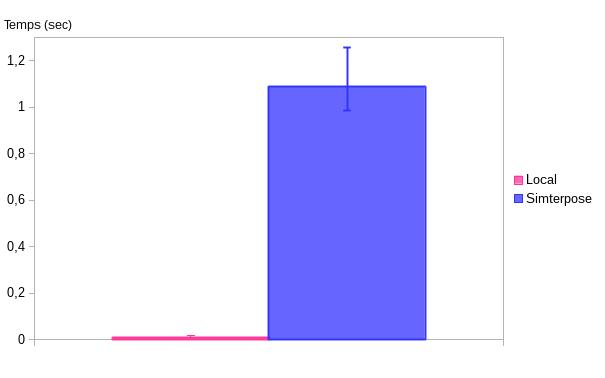
\includegraphics[scale=0.5]{mesures/graph/Bigmsg_local.jpg}
    \caption{Temps d'exécution lors de l'envoi d'un message de 1Mo avec et sans Simterpose.}
    \label{Network_Big_Local}
\end{figure}

\begin{figure}
  \centering
    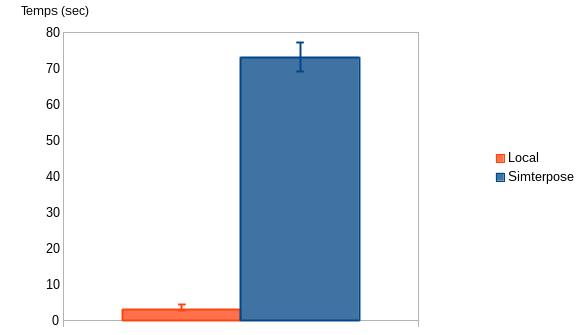
\includegraphics[scale=0.5]{mesures/graph/Littlemsg_local.jpg}
    \caption{Temps d'exécution lors de l'envoi d'un million de messages de 128o avec et sans Simterpose.}
    \label{Network_Little_Local}
\end{figure}

Dans le cas de l'envoi de plusieurs petits messages le temps moyen d'exécution en local est d'environ 3 secondes, avec Simterpose il est de 72 secondes en \textit{full mediation} et de 75 secondes en \textit{address translation}.

Lors de l'envoi d'un gros message le temps d'exécution moyen est de 0,01 secondes pour exécuter l'application en local alors qu'avec Simterpose il oscille entre 1 et 1,1 secondes selon le type de médiation.

\paragraph{Quelle médiation pour quel type d'application}
 Cette seconde expérience vise à comparer les deux médiations que nous avons implémentés. Pour cela, en suivant le protocole présenté plus haut on va exécuter les deux applications réseau choisi en utilisant les deux types de médiations. Les résultats de notre expérience sont présentés Figures \ref{Network_Big_Mediation} et \ref{Network_Little_Mediation}.

 \begin{figure}[H]
  \centering
    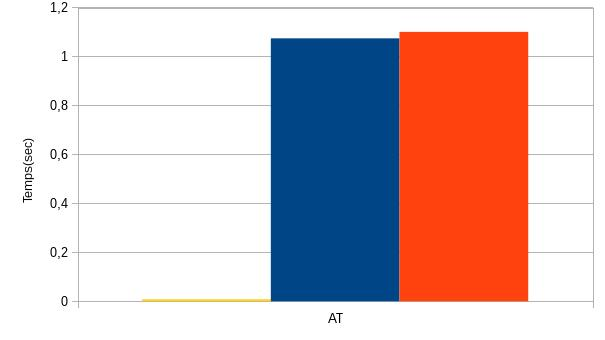
\includegraphics[scale=0.5]{mesures/graph/Bigmsg.jpg}
    \caption{Temps d'exécution lors de l'envoi d'un message de 1Mo en \textit{full mediation} et \textit{address translation}.}
    \label{Network_Big_Mediation}
\end{figure}

\begin{figure}[H]
  \centering
    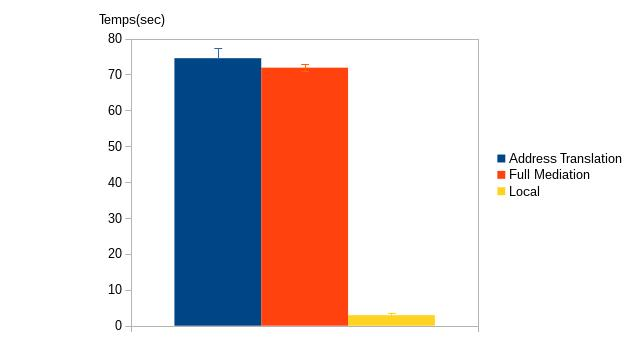
\includegraphics[scale=0.5]{mesures/graph/Littlemsg.jpg}
    \caption{Temps d'exécution lors de l'envoi d'un million de messages de 128o en \textit{full mediation} et \textit{address translation}avec et sans Simterpose.}
    \label{Network_Little_Mediation}
\end{figure}

Lors de l'envoi de nombreux petits messages, on peut constater que la \textit{full mediation} est plus rapide que l'\textit{address translation} avec un écart moyen de 3\%.

Lorsque l'on envoie un gros message, on constate que l'écart moyen entre les deux types de médiation est de 2.5\%.

\subsubsection{Analyse}
\paragraph{Overhead concernant le temps d'exécution}
Si l'on souhaite réellement mettre en place notre émulateur, dans le cas de l'envoi de plusieurs petits messages, l'exécution prendra 25 fois plus de temps et lors de l'envoi d'un gros message, elle prendra 100 fois plus de temps. Cet écart s'explique par les nombreux appels systèmes et changements de contexte que nécessite Simterpose de par son utilisation coûteuse de \texttt{ptrace} en plus de l'exécution de l'appel système lui-même lorsqu'on utilise l'\textit{address translation}. Cette expérience constitue cependant le pire scénario possible, avec un très grand nombre de petits messages échangés dans l'application.

\paragraph{Quelle médiation pour quel type d'application}
Lorqu'on utilise l'\textit{address translation} l'envoi de messages génère des appels systèmes et changements de contexte qui n'ont pas lieu en \textit{full mediation} puisque dans ce cas, comme nous l'avons expliqué en section \ref{paragraph:FULL_MEDIATION}, les appels systèmes ne sont pas exécutés. Ces derniers étant coûteux cela explique pourquoi l'\textit{address translation} est moins rapide. De plus, en \textit{full mediation}, même si les appels systèmes sont bloqués, nous utilisons l'appel système \texttt{ptrace} pour effectuer nous-même les appels demandés par l'application que nous avons bloqués. Cette méthode même si elle reste moins coûteuse que l'exécution de l'appel système demandé consomme des cycles CPU, ce qui explique le faible écart entre les temps d'exécution moyen des deux types de médiation.

Nous pensons que lors de l'envoi d'un gros message l'\textit{address translation} est légèrement plus rapide car nous envoyons un seul message de 1Mo de données. En effet, même si en \textit{full mediation} on a beaucoup moins de changement de contexte de par le blocage des appels systèmes ici on ne fait qu'un seul appel et la faible différence entre les deux médiations ne peut donc être dû à cela. Par contre, lors de l'envoi d'un tel message il faut prendre en compte la gestion de la mémoire car le message doit être stocké avant de pouvoir être envoyé par morceau sur le réseau. Ainsi, si on ne gère pas la mémoire de façon efficace on surconsomme des cycles CPU lorsqu'on accède à cette dernière. Or, nous n'avons pas encore mis en place de politique de gestion de mémoire particulière pour Simterpose. Néanmoins, les résultats ont une plus grande variabilité des temps d'exécution en \textit{address translation} qu'en \textit{full mediation}. On peut donc supposer qu'avec une politique de gestion mémoire aussi efficace que celle qui est utilisée par le système la \textit{full mediation} serait probablement plus rapide que l'\textit{address translation} comme dans l'expérience précédente.

 Ainsi, lors de l'envoi de nombreux messages il vaut mieux privilégier la \textit{full mediation}. De plus, les deux médiations se valent lorsqu'on souhaite envoyer de gros messages.
\subsubsection{Conclusion}

Pour notre première expérience, le sur-coût mesuré est certes important, mais indique que notre approche reste utilisable même dans ce cas.

De plus, pour notre seconde expérience la faible durée d'exécution d'une expérience nous permet de considérer que l'\textit{overhead} dû à la mise en place de Simterpose est acceptable.

Ainsi, nous pouvons connclure que ce type de virtualisation est possible pour le réseau.
